%% Prezentace: Aplikace fuzzy a pravděpodobnostních automatů
%% Martin Jašek, UPOL
%% 31. května 2018, 
%%
%% Vygenerováno programem plain2beamer 1.2
%%%%%%%%%%%%%%%%%%%%%%%%%%%%%%%%%%%%%%%%%%%%%%%%%%%%%%%%%%%%%%%%%%%%%%%%%%%%%%
\documentclass{beamer}
\usepackage[czech]{babel}
\usepackage[utf8x]{inputenc}
%%%%%%%%%%%%%%%%%%%%%%%%%%%%%%%%%%%%%%%%%%%%%%%%%%%%%%%%%%%%%%%%%%%%%%%%%%%%%%
\title{Aplikace fuzzy a pravděpodobnostních automatů}
\author{Martin Jašek}
\date{31. května 2018}
\institute{UPOL}
%%%%%%%%%%%%%%%%%%%%%%%%%%%%%%%%%%%%%%%%%%%%%%%%%%%%%%%%%%%%%%%%%%%%%%%%%%%%%%
\mode<presentation> {
  \usetheme{Rochester}
  \usecolortheme{whale}
}
%%%%%%%%%%%%%%%%%%%%%%%%%%%%%%%%%%%%%%%%%%%%%%%%%%%%%%%%%%%%%%%%%%%%%%%%%%%%%%
\begin{document}
%%%%%%%%%%%%%%%%%%%%%%%%%%%%%%%%%%%%%%%%%%%%%%%%%%%%%%%%%%%%%%%%%%%%%%%%%%%%%%
\begin{frame}	%% Slajd 1 - Úvodní slajd
	\titlepage
\end{frame}

%%%%%%%%%%%%%%%%%%%%%%%%%%%%%%%%%%%%%%%%%%%%%%%%%%%%%%%%%%%%%%%%%%%%%%%%%%%%%%
\begin{frame}	%% Slajd 3 - Úvod
\frametitle{Úvod}
\begin{itemize}
	\item fuzzy automaty kombinují automaty a fuzzy množiny
	\item obdobně pravděpodobnostní automaty
	\item neurčitost $\Rightarrow$ reálný svět
\end{itemize}
\end{frame}

%%%%%%%%%%%%%%%%%%%%%%%%%%%%%%%%%%%%%%%%%%%%%%%%%%%%%%%%%%%%%%%%%%%%%%%%%%%%%%
\begin{frame}	%% Slajd 4 - Fuzzy automat
\frametitle{Fuzzy automat}
\begin{definition}[Nedeterministický fuzzy automat]\label{def-ZaklDefNedFuzzAut}
 Nedeterministický fuzzy automat $\mathbf{A}$ je pětice $(Q, \Sigma, \mu, \sigma, \eta)$, kde $Q$ je konečná množina stavů, $\Sigma$ je abeceda, $\mu$ je fuzzy přechodová funkce (fuzzy relace $Q \times \Sigma \times 2^Q \rightarrow [0, 1]$) a $\sigma$ a $\eta$ jsou po řadě fuzzy množiny nad $Q$ počátačních, resp. koncových stavů.
\end{definition}
\end{frame}

%%%%%%%%%%%%%%%%%%%%%%%%%%%%%%%%%%%%%%%%%%%%%%%%%%%%%%%%%%%%%%%%%%%%%%%%%%%%%%
\begin{frame}	%% Slajd 5 - 
\frametitle{}
\centering 
\includegraphics{fa-example}
%TODO výpočet
\end{frame}

%%%%%%%%%%%%%%%%%%%%%%%%%%%%%%%%%%%%%%%%%%%%%%%%%%%%%%%%%%%%%%%%%%%%%%%%%%%%%%
\begin{frame}	%% Slajd 6 - Deformace automatu
\frametitle{Deformace automatu}
\centering
\includegraphics[width=0.9\textwidth]{deformed}
%TODO metodika?
\end{frame}

%%%%%%%%%%%%%%%%%%%%%%%%%%%%%%%%%%%%%%%%%%%%%%%%%%%%%%%%%%%%%%%%%%%%%%%%%%%%%%
\begin{frame}	%% Slajd 7 - Detekce a korekce překlepů
\frametitle{Detekce a korekce překlepů}
\centering
\begin{tabular}{|l|l|}
 \hline
 vstup 			&	výstup	\\
 \hline
 februacy	 	& february	\\
 jaruanry		& january		\\
 devmber		 	& december	\\
 october			& october		\\
 asdbril			& april			\\
 maj					& march			\\
 jana				& may				\\
 poctober		& october		\\
 asauguszt		& august		\\
 mnobmvmert	& november 	\\
 \hline
\end{tabular}
%\begin{tabular}{|l||l|l|l|l|l|l|l|l|l|}
%  \hline
%  vstup 	& februacy & jaruanry & devmber  & october & asdbril	\\\hline
%  výstup 	& february & january  & december & october & april	\\\hline
%  \hline
%  vstup 	& maj   & jana & poctober & asauguszt  & mnobmvmert	\\\hline
%  výstup	& march & may  & october  & august     & november	\\\hline
%\end{tabular}
\end{frame}

%%%%%%%%%%%%%%%%%%%%%%%%%%%%%%%%%%%%%%%%%%%%%%%%%%%%%%%%%%%%%%%%%%%%%%%%%%%%%%
\begin{frame}	%% Slajd 8 - Rozpoznávání ručně psaného textu
\frametitle{Rozpoznávání ručně psaného textu}
\centering
\includegraphics{handwritten-principle}
\end{frame}

%%%%%%%%%%%%%%%%%%%%%%%%%%%%%%%%%%%%%%%%%%%%%%%%%%%%%%%%%%%%%%%%%%%%%%%%%%%%%%
\begin{frame}	%% Slajd 9 - Ukázka aplikace
\frametitle{Ukázka aplikace}
\centering
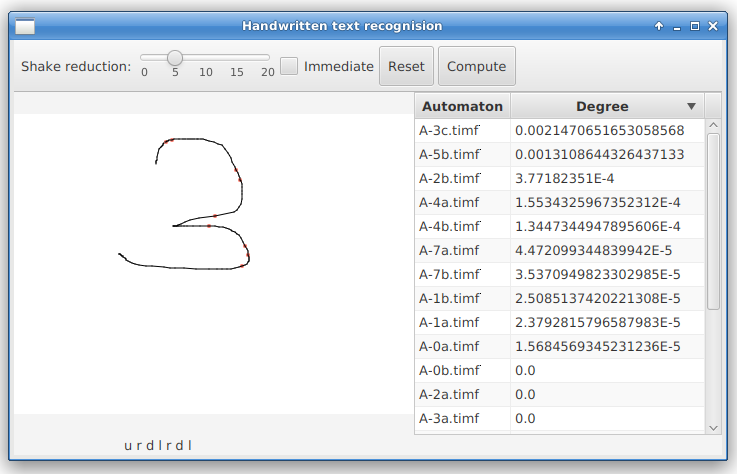
\includegraphics[width=0.9\textwidth]{handwritten-screen}
\end{frame}

%%%%%%%%%%%%%%%%%%%%%%%%%%%%%%%%%%%%%%%%%%%%%%%%%%%%%%%%%%%%%%%%%%%%%%%%%%%%%%
\begin{frame}	%% Slajd 10 - Rozpoznávání složených geometrických tvarů
\frametitle{Rozpoznávání složených geometrických tvarů}
\centering
\includegraphics{composite-shape}
\end{frame}

%%%%%%%%%%%%%%%%%%%%%%%%%%%%%%%%%%%%%%%%%%%%%%%%%%%%%%%%%%%%%%%%%%%%%%%%%%%%%%
\begin{frame}	%% Slajd 11 - Odstranění šumu
\frametitle{Odstranění šumu}
\centering

\includegraphics{noises-my}
\vfill \pause
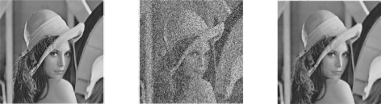
\includegraphics{noises-cited}
\let\thefootnote\relax\footnote[1]{SADEGHI, Sana; REZVANIAN, Alireza; KAMRANI, Ebrahim. An efficient method for impulse noise reduction from images using fuzzy cellular Automata. \textit{International Journal of Electronics and Communications.} 2012.}
\end{frame}

%%%%%%%%%%%%%%%%%%%%%%%%%%%%%%%%%%%%%%%%%%%%%%%%%%%%%%%%%%%%%%%%%%%%%%%%%%%%%%
\begin{frame}	%% Slajd 12 - Monitorování elektrických sítí
\frametitle{Monitorování elektrických sítí}
\centering
\includegraphics{electrics}
\end{frame}

%%%%%%%%%%%%%%%%%%%%%%%%%%%%%%%%%%%%%%%%%%%%%%%%%%%%%%%%%%%%%%%%%%%%%%%%%%%%%%
\begin{frame}	%% Slajd 13 - Metoda lisování dat
\frametitle{Metoda lisování dat}
\begin{itemize}
	\item mějme tabulku záznamů (tzv. trénovací množinu) $(x_1, \dots x_n, y) \in T \subseteq \{0, 1\}^{n+1}$
	\item označme $\mathcal{L}_y$ množinu řetězců $x_1 \dots x_n$ takových, že $(x_1, \dots x_n, y) \in T$
	\item sestavme fuzzy automat $\mathbf{A}$ rozpoznávající $\mathcal{L}_y$
	\item fuzzy minimalizací automatu $\mathbf{A}$ s parametrem $0 \leq \delta \leq 1$ obdržíme automat $\mathbf{A}'$
	\item automat $\mathbf{A}'$ slouží jako model klasifikující sekvence $(x_1 \dots x_n)$
\end{itemize}
\end{frame}

%%%%%%%%%%%%%%%%%%%%%%%%%%%%%%%%%%%%%%%%%%%%%%%%%%%%%%%%%%%%%%%%%%%%%%%%%%%%%%
\begin{frame}	%% Slajd 14 - Závěr
\frametitle{Závěr}
\begin{itemize}
	\item fuzzy automaty nacházejí uplatnění v praxi
	\item přinášejí elegantní řešení
	\item často je nutná složitá příprava dat
	\item složitost vs. správnost
\end{itemize}
\end{frame}

%%%%%%%%%%%%%%%%%%%%%%%%%%%%%%%%%%%%%%%%%%%%%%%%%%%%%%%%%%%%%%%%%%%%%%%%%%%%%%
\begin{frame}	%% Slajd 15 - 
\frametitle{}
\begin{center}
\huge{Děkuji za pozornost}
\vfill
\includegraphics{bye}
\end{center}
\end{frame}

\end{document}
